%-------------------------------------------------------------------------
% introduction.tex
%-------------------------------------------------------------------------

%-------------------------------------------------------------------------
\setjobnamebeamerversion{introductionSlide}

\usetheme{Enib}
%-------------------------------------------------------------------------

%-------------------------------------------------------------------------
\newtheorem{rem}{Remarque}[section]
\newtheorem{defin}{Définition}[section]
\newtheorem{td}{\color{blue}TD}[section]
%-------------------------------------------------------------------------

%-------------------------------------------------------------------------
\lstset
{
language=Python,
basicstyle=\ttfamily,
identifierstyle=\ttfamily,
keywordstyle=\color{blue}\ttfamily,
commentstyle=\color{gray}\ttfamily,
stringstyle=\color{green}\ttfamily,
showstringspaces=false,
extendedchars=true,
numbers=left, 
numberstyle=\tiny,
frame=lines,
linewidth=0.95\textwidth,
xleftmargin=5mm
} 
%-------------------------------------------------------------------------

%-------------------------------------------------------------------------
\def\exo#1{\mbox{}\ \hfill\mbox{\color{blue}$\rule{2mm}{2mm}\,$\footnotesize\sc TD\ref{#1}}}
\def\exercice#1#2{\mbox{}\ \ TD \ref{#1}\ #2\ \dotfill\ \pageref{#1}\mbox{}}

\newenvironment{py}[1]{\begin{minipage}[t]{#1}\footnotesize}{\end{minipage}}
%-------------------------------------------------------------------------

%-------------------------------------------------------------------------
\title[Algorithmique]{\bf Initiation à l'algorithmique}
\subtitle{\bf --- introduction générale ---}

\author[\tt jacques.tisseau@enib.fr]{\large\bf Jacques TISSEAU}
\institute[\enib]{{\large\enib--\cerv}}
\date[enib\copyright 2009-2014]{\footnotesize enib\copyright 2009-2014}
%-------------------------------------------------------------------------

\graphicspath{{../../fig/}}


%-------------------------------------------------------------------------
\begin{document}
%-------------------------------------------------------------------------

%------------------------------------------
\begin{frame}
\frametitle{\uppercase{Informatique \hfill {S1}}}
%------------------------------------------
\titlepage

\end{frame}
\note{
\mbox{}\null\vfill

\begin{rem}[Notes de cours : couverture]
Ce support de cours accompagne le 
chapitre 1 des notes de cours « Initiation à l'algorithmique ».
$$\fbox{
\includegraphics[width=10cm,page=1]{../../../pdf/cours/info-S1.pdf}}$$
\end{rem}
}
%------------------------------------------

%------------------------------------------
\begin{frame}
\frametitle{\uppercase{Informatique}}
\framesubtitle{\uppercase{Définitions}}
%------------------------------------------
\begin{block}{Définition}
\begin{itemize}
\item \alert{\bf infor}mation auto\alert{\bf matique}\hfill
		(P. Dreyfus, 1962)
%\pause
\item {\bf informatique} : science du traitement automatique de l'information
\end{itemize}
\end{block}
%\pause
\begin{block}{Matériel $\leftrightarrow$ Logiciel}
\begin{itemize}
\item matériel : ordinateurs\hfill (J. Perret, 1955)

	\centerline{
\includegraphics[width=3cm]{ordibureau.jpg}}
%\pause
\item logiciel : ensemble de programmes remplissant une fonction déterminée,
	permettant l'accomplissement d'une tâche donnée
\end{itemize}
\end{block}

\end{frame}
\note{
{\bf Définitions}\begin{description}
\item[informatique]
L'informatique est la science du traitement automatique de l'information.
\item[matériel]
Le matériel informatique est un ensemble de dispositifs physiques utilisés pour traiter
automatiquement des informations.
\item[logiciel]
Le logiciel est un ensemble structuré d'instructions décrivant un traitement d'informations
à faire réaliser par un matériel informatique.
\end{description}
\null\vfill

\begin{rem}[Cours Informatique S1]
Dans ce cours, nous ne nous intéresserons qu'aux aspects logiciels de l'informatique.
\end{rem}
}
%------------------------------------------

%------------------------------------------
\begin{frame}
\frametitle{\uppercase{Ordinateur}}
\framesubtitle{\uppercase{Architecture de Von Neumann}}
%------------------------------------------
%\centerline{\multiinclude[graphics={width=8cm},format=pdf]{ordinateur}}
\centerline{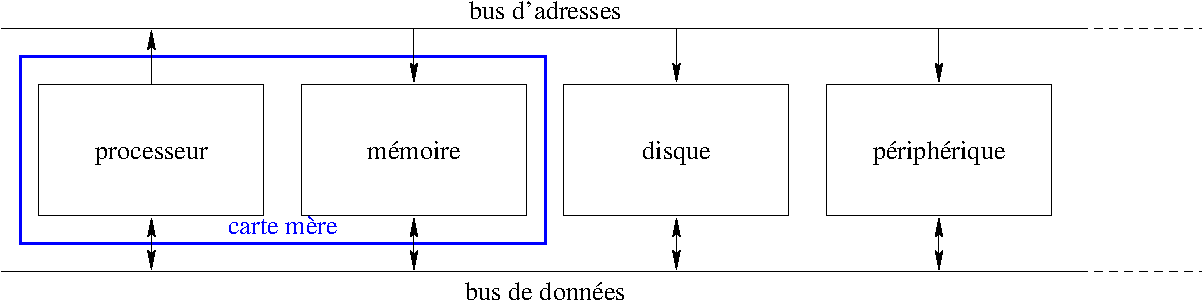
\includegraphics[width=8cm]{ordinateur.pdf}}
%\pause
\begin{block}{Architecture de Von Neumann}
\begin{itemize}
\item élément central : processeur (unité arithmétique et logique, unité de contrôle)
\item échanges avec les autres composants : stocker, récupérer
	et transférer des données
\item bus d'adresse : désigner le composant
\item bus de données : véhiculer l'information
\end{itemize}
\end{block}
\end{frame}
\note{
{\bf Définitions}\begin{description}
\item[bit] Un bit est un chiffre binaire (0 ou 1). 
C'est l'unité élémentaire d'information.
\item[octet] Un octet est une unité d'information composée de 8 bits.
\end{description}
\null\vfill

\begin{td}[Unités d'information]
Combien y a-t-il d'octets dans 1 ko (kilooctet), 
1 Go (gigaoctet), 1 To (téraoctet), 1 Po (pétaoctet), 1 Eo (exaoctet),
1 Zo (zettaoctet) et 1 Yo (yottaoctet) ?
\end{td}

\begin{td}[Stockage de données]
Donner l'ordre de grandeur en octets pour stocker en mémoire :
une page d'un livre,
une encyclopédie en 20 volumes,
une photo couleur,
une heure de vidéo,
une minute de son,
une heure de son.
\end{td}
}
%------------------------------------------

%------------------------------------------
\begin{frame}
\frametitle{\uppercase{Ordinateurs}}
\framesubtitle{\uppercase{Exemples}}
%------------------------------------------
\begin{columns}
\column{5.5cm}
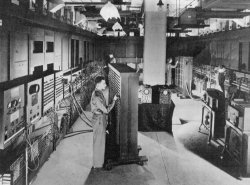
\includegraphics[width=5cm]{eniac2.jpg}
%\pause

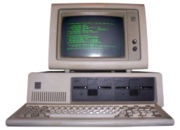
\includegraphics[width=2.75cm]{ibmpc.jpg}
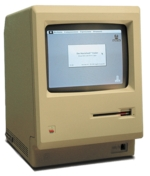
\includegraphics[width=2.75cm]{macintosh.jpg}
%\pause

\column{5.5cm}
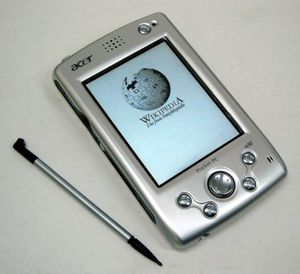
\includegraphics[width=2.75cm]{pda.jpg}\hfill
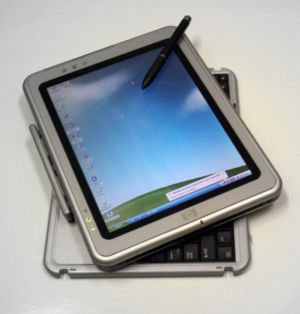
\includegraphics[width=2.75cm]{tablette.jpg}

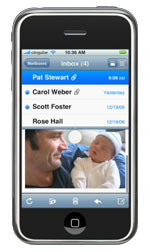
\includegraphics[width=2.5cm]{iphone.jpg}\hfill
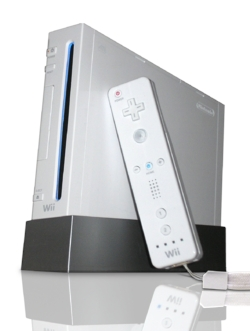
\includegraphics[width=3cm]{wii.jpg}

\end{columns}
\end{frame}
\note{
{\bf Définitions}\begin{description}
\item[MIPS] 
	Le MIPS est l'unité de mesure qui représente un million d'instructions par seconde.
\item[FLOPS] 
	Le FLOPS (Floating-point Operations Per Second) est l'unité de mesure
	qui représente le nombre d'opérations à virgule flottante par seconde.
\end{description}
\mbox{}\null\vfill

\begin{td}[Puissance de calcul]
Donner l'ordre de grandeur en instructions par seconde des machines suivantes :
le premier micro-ordinateur de type PC,
une console de jeu actuelle,
un micro-ordinateur actuel,
{\em Deeper-Blue} : l'ordinateur qui a « battu » Kasparov aux échecs en 1997,
le plus puissant ordinateur actuel.
\end{td}
}
%------------------------------------------

%------------------------------------------
\begin{frame}
\frametitle{\mbox{\uppercase{Micro-processeurs Intel}}}
\framesubtitle{\uppercase{Exemples}}
%------------------------------------------
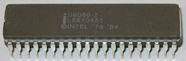
\includegraphics[width=3.25cm]{8086.jpg}\hfill
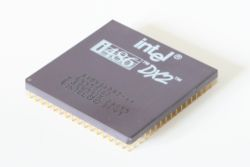
\includegraphics[width=3.25cm]{80486.jpg}

\mbox{}\hfill 8086 \hfill 80486 \hfill \mbox{}
%\pause
\null\vfill

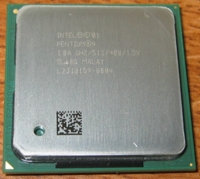
\includegraphics[width=3.25cm]{pentium4.jpg}\hfill
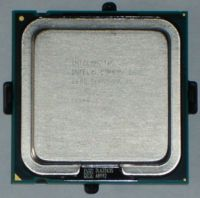
\includegraphics[width=3.25cm]{core2.jpg}


\mbox{}\hfill Pentium 4 \hfill Core Duo \hfill \mbox{}
\end{frame}
\note{
\mbox{}\null\vfill

\begin{rem}[Loi de Moore]
	Gordon Earl Moore est le co-fondateur avec Robert Noyce et Andrew Grove de la société Intel en 1968 
	(fabriquant n$^{\circ}$1 mondial de microprocesseurs).
	En 1965, il expliquait que la complexité des semiconducteurs 
	doublait tous les dix-huit mois à coût constant depuis 1959, date de leur invention. 
	En 1975, il précise sa «~première loi~» en affirmant que le nombre de transistors des microprocesseurs  
	sur une puce de silicium double tous les deux ans («~deuxième loi~»).
	
	\centerline{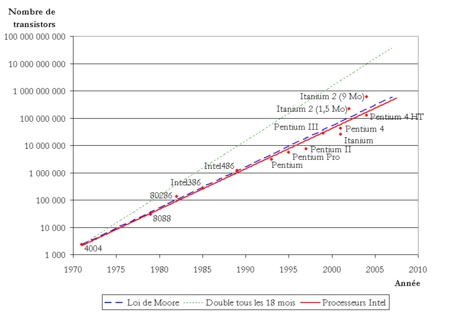
\includegraphics[width=8cm]{loimoore.jpg}}
	\end{rem}}
%------------------------------------------

%------------------------------------------
\begin{frame}
\frametitle{\mbox{\uppercase{Algorithmique}}}
\framesubtitle{\uppercase{Définitions}}
%------------------------------------------
\begin{block}{Algorithme}
\begin{itemize}
\item mathématicien persan du $9^{\grave eme}$ siècle
	\alert{Al-Khwarizmi}
%\pause
\item méthode de calcul qui indique la démarche à suivre
	pour résoudre une série de problèmes équivalents
	en appliquant dans un ordre précis une suite finie
	de règles
\end{itemize}
\end{block}
%\pause

\begin{block}{Algorithmique}
\begin{itemize}
\item art de construire des algorithmes
%\pause
\item validité, robustesse, réutilisabilité
%\pause
\item complexité, efficacité
\end{itemize}
\end{block}

\end{frame}
\note{
{\bf Définitions}\begin{description}
\item[algorithme]
	Un algorithme est une suite ordonnée d'instructions qui indique la démarche 
	à suivre pour résoudre une série de problèmes équivalents.
\item[algorithmique]
	L'algorithmique est la science des algorithmes.
	\vspace*{1cm}
\item[validité]
	La validité d'un algorithme est son aptitude à réaliser exactement la tâche
	pour laquelle il a été conçu.
\item[robustesse]
	La robustesse d'un algorithme est son aptitude à se protéger de conditions 
	anormales d'utilisation.
\item[réutilisabilité]
	La réutilisabilité d'un algorithme est son aptitude à être réutilisé pour résoudre
	des tâches équivalentes à celle pour laquelle il a été conçu.
\item[complexité]
	La complexité d'un algorithme est le nombre d'instructions élémentaires à exécuter pour
	réaliser la tâche pour laquelle il a été conçu.
\item[efficacité]
	L'efficacité d'un algorithme est son aptitude à utiliser de manière optimale
	les ressources du matériel qui l'exécute.
\end{description}
}
%------------------------------------------

%------------------------------------------
\begin{frame}
\frametitle{\mbox{\uppercase{Du problème au code source}}}
\framesubtitle{\uppercase{Algorithmique et programmation}}
%------------------------------------------
\begin{columns}
\column{4cm}
%$$\multiinclude[graphics={height=6.75cm},format=pdf]{informatique}$$
$$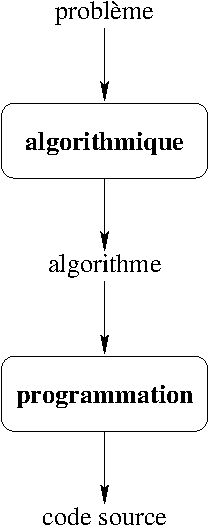
\includegraphics[height=6.75cm]{informatique.pdf}$$
%\pause
\column{8cm}
\begin{itemize}
\item Un algorithme exprime la structure logique d'un programme :
	il est indépendant du langage de programmation.
	\vspace*{1.5cm}
%\pause
\item La traduction de l'algorithme dans un langage de programmation
	dépend du langage choisi.
\end{itemize}
\end{columns}

\end{frame}
\note{
\mbox{}\null\vfill

\begin{td}[Dessins sur la plage : exécution]
On cherche à faire dessiner une figure géométrique sur la plage 
à quelqu'un qui a les yeux bandés.
Quelle figure géométrique dessine-t-on en exécutant la suite d'instructions 
suivante : 
avance de 10 pas,
tourne à gauche d'un angle de $120^\circ$,
avance de 10 pas,
tourne à gauche d'un angle de $120^\circ$, 
avance de 10 pas ?
\end{td}

\begin{td}[Dessins sur la plage : conception]
Faire dessiner une spirale rectangulaire de 5 côtés, le plus petit côté
faisant 2 pas de long et chaque côté fait un pas de plus que le précédent.
\end{td}

\begin{td}[Mon premier programme en {\sc Python}]
Ecrire en {\sc Python} l'algorithme de la spirale rectangulaire à 5 côtés.
\end{td}
}
%------------------------------------------

%------------------------------------------
\begin{frame}
\frametitle{\mbox{\uppercase{Du code source à l'exécution}}}
\framesubtitle{\uppercase{Compilation versus interprétation}}
%------------------------------------------
%$$\multiinclude[graphics={height=6.75cm},format=pdf]{compilateur}$$
$$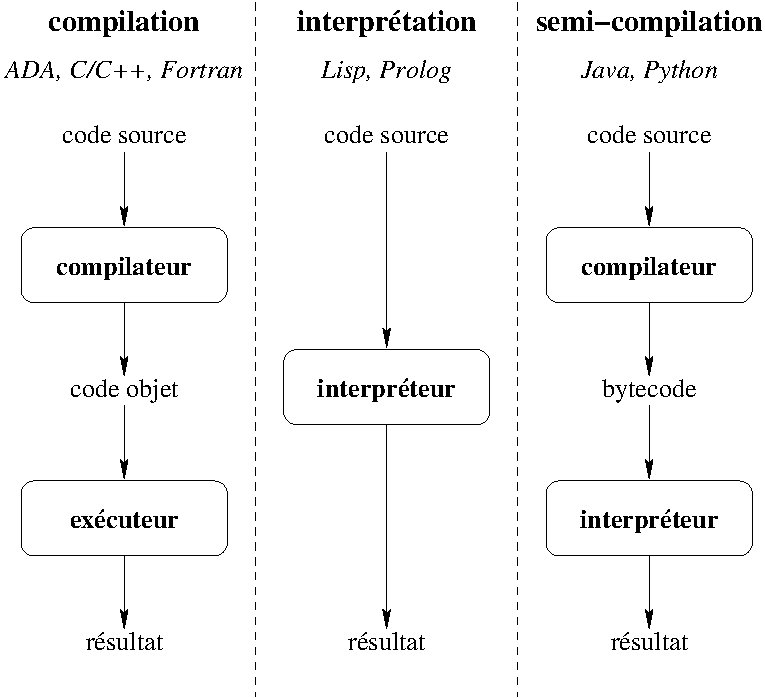
\includegraphics[height=6.75cm]{compilateur.pdf}$$

\end{frame}
\note{
{\bf Définitions}\begin{description}
\item[compilateur] 
	Un compilateur est un programme informatique qui traduit un langage, 
	le langage source, en un autre, appelé le langage cible. 

	Un compilateur sert le plus souvent à traduire un code source écrit 
	dans un langage de programmation en un autre langage, habituellement un langage
 	d'assemblage ou un langage machine. Le programme en langage machine produit par 
	un compilateur est appelé code objet.
\item[interpréteur]
	Un interpréteur est un outil informatique (logiciel ou matériel) ayant pour tâche 
	d'analyser et d'exécuter un programme écrit dans un langage source.
\end{description}
\mbox{}\null\vfill

\begin{td}[Première utilisation de {\sc Python}]
\begin{enumerate}
\item Lancer {\sc Python}.
\item Utiliser {\sc Python} comme une simple calculette.
\item Exécuter l'algorithme de la spirale rectangulaire à 5 côtés.
\item Quitter {\sc Python}.
\end{enumerate}
\end{td}
}
%------------------------------------------

%------------------------------------------
\begin{frame}
\frametitle{\uppercase{Objectifs thématiques}}
\framesubtitle{\uppercase{Algorithmique et Python}}
%------------------------------------------
\begin{block}{Objectifs}
acquérir les notions fondamentales de l'\alert{algorithmique}
et les mettre en \oe uvre avec un langage opérationnel (\alert{\python}).
\end{block}
%\pause
\begin{block}{Pré-requis}
	\begin{itemize}
	\item Bac scientifique
	\end{itemize}
\end{block}
%\pause
\begin{block}{3 objectifs majeurs}
\begin{enumerate}
\item instructions de base
%\pause
\item procédures et fonctions
%\pause
\item structures de données linéaires
\end{enumerate}
\end{block}

\end{frame}
\note{
\mbox{}\null\vfill

\begin{rem}[Objectifs thématiques]
Plus précisément, nous étudierons successivement :
\begin{enumerate}
\item les instructions de base permettant de décrire les algorithmes : affectation, tests, boucles;
\item les procédures et les fonctions qui permettent de structurer et de réutiliser les algorithmes;
	on parlera alors d'encapsulation, de préconditions, de portée des variables, de passage de paramètres,
	d'appels de fonctions, de récursivité et de jeux de tests;
\item les structures de données linéaires : tableaux, listes, piles, files, qui améliorent la
	structuration des données manipulées par les algorithmes. A cette occasion, on évaluera
	la complexité et l'efficacité de certains algorithmes utilisant ces structures linéaires.
\end{enumerate}
Ces différentes notions seront mise en \oe uvre à travers l'utilisation du 
langage {\sc Python}.
\end{rem}
}
%------------------------------------------

%------------------------------------------
\begin{frame}
\frametitle{\uppercase{Objectifs pédagogiques}}
\framesubtitle{\uppercase{Métaphore musicale}}
%------------------------------------------
\begin{block}{Faire ses gammes}
	\begin{itemize}
	\item apprentissage d'un langage algorithmique (semestre 1)
	\item pédagogie par objectifs
	\end{itemize}
\end{block}
%\pause
\begin{block}{Jouer les grands classiques}
	\begin{itemize}
	\item apprentissage des algorithmes classiques (semestres 1 et 2)
	\item pédagogie par l'exemple
	\end{itemize}
\end{block}
%\pause
\begin{block}{Composer ses propres morceaux}
	\begin{itemize}
	\item apprentissage de la conception d'algorithmes (semestre 2)
	\item pédagogie par problèmes
	\end{itemize}
\end{block}

\end{frame}
\note{
\mbox{}\null\vfill

\begin{rem}[Taxonomie de Bloom]
Benjamin Bloom (1913-1999) psychologue amé\-ri\-cain spécialisé en pédagogie.

\centerline{\begin{tabular}{|l|l@{ : }p{5.5cm}|}
\hline
{\bf S1}& \bf Connaître   & définir, distinguer, acquérir, identifier, rappeler, reconnaître\ldots \\
 	& \bf Comprendre  & traduire, illustrer, représenter, dire avec ses mots, 
		distinguer, réécrire, réarranger, expliquer, démontrer\ldots \\
 	& \bf Appliquer   & appliquer, généraliser, relier, choisir, développer, 
				utiliser, employer, 
		 		transférer, classer, restructurer\ldots \\
\hline
{\bf S2}& \bf Analyser    & distinguer, détecter, classer, reconnaître, catégoriser, 
			déduire, discerner, comparer\ldots \\
 	& \bf Synthétiser & écrire, relater, produire, constituer, transmettre, modifier, créer, 
		 	proposer, planifier, projeter, spécifier, combiner, 
			classer, formuler\ldots \\
 	& \bf Evaluer     & juger, argumenter, valider, décider, comparer\ldots \\
\hline
\end{tabular}}
\end{rem}
}
%------------------------------------------

%------------------------------------------
\begin{frame}
\frametitle{\mbox{\uppercase{Objectifs comportementaux}}}
\framesubtitle{\uppercase{Rigueur, persévérance, autonomie}}
%------------------------------------------
\begin{block}{Savoir-être}
	\begin{itemize}
	%\item<1-> \alert{rigueur}
	\item \alert{rigueur}
	
		\mbox{}\hfill {\em respect des consignes, précision,
		exactitude}\\
		\mbox{}\hfill écrit $\leftrightarrow$ image

	%\item<2-> \alert{persévérance}
	\item \alert{persévérance}
	
		\mbox{}\hfill {\em aller au bout des choses}\\
		\mbox{}\hfill finir $\leftrightarrow$  papillonner

	%\item<3-> \alert{autonomie}
	\item \alert{autonomie}
	
		\mbox{}\hfill {\em pratique personnelle, autoformation}\\
		\mbox{}\hfill initiatives $\leftrightarrow$ assistances
	\end{itemize}
\end{block}

\end{frame}
\note{
{\bf Définitions}\begin{description}
\item[rigueur] La rigueur est la qualité de celui qui agit avec précision, exactitude, 
	en respectant une logique inflexible.
\item[persévérance] La persévérance est la qualité de celui qui s'attache avec détermination 
	et constance à mener à bien ce qu'il a entrepris. 
\item[autonomie] L'autonomie est la qualité de celui qui est capable
	d'agir sans intervention extérieure.
\end{description}
\null\vfill

\begin{td}[Rigueur : erreur de syntaxe en {\sc Python}]
On considère la session {\sc Python} suivante :\\[1mm]
\mbox{}\hfill\begin{minipage}{7cm}\tt
>>> x = 3\\
>>> \ y = x\\
\mbox{}\ \ File "<stdin>", line 1\\
\mbox{}\ \ \ \ y = x\\
\mbox{}\ \ \ \ \char`^\\
{\color{red}SyntaxError: invalid syntax}\\
>>>
\end{minipage}\\[1mm]
De quelle erreur de syntaxe s'agit-il ?
\end{td}
\begin{td}[Persévérance : dessins sur la plage]
Finir l'algorithme suivant qui cherche à dessiner un losange sur la plage :\\
avance de 10 pas, \ldots
\end{td}
}
%------------------------------------------

%------------------------------------------
\begin{frame}
\frametitle{\uppercase{Planning}}
\framesubtitle{\uppercase{Page Web sur} \tt moodle.enib.fr}
%------------------------------------------
\begin{block}{Horaires}
	\begin{itemize}
	\item \alert{Cours/TD} : 21h (1$\times$ 1h30 chaque semaine) 
		en salle banalisée
	\item \alert{TD} : 21h (1$\times$ 3h toutes les 2 semaines) 
		en salle informatique
	\end{itemize}
\end{block}
%\pause
\begin{block}{Planning prévisionnel}
Voir \href{https://moodle.enib.fr/course/view.php?id=24}{site Web}  \hfill ENT -- Informatique S1
\end{block}
\end{frame}
\note{
\mbox{}\null\vfill

\begin{rem}[Exemple de planning prévisionnel]
Les enseignements d'Informatique S1 de l'ENIB s'étalent sur 14 semaines
à raison de 3h de cours toutes les 2 semaines en alternance avec 3h 
de laboratoire toutes les 2 semaines.
$$\begin{tabular}{|l|p{4cm}|p{4cm}|p{4cm}|}
\cline{2-3}
\multicolumn{1}{c|}{} & \bf Cours & \bf Laboratoire \\
\hline
\bf 1 & instructions de base & --- \\
\hline
\bf 2 & --- & instructions de base \\
\hline
\bf 3 & instructions de base & --- \\
\hline
\bf 4 & --- & instructions de base \\
\hline
\bf 5 & instructions de base & --- \\
\hline
\bf 6 & --- & instructions de base \\
\hline
\bf 7 & procédures et fonctions & --- \\
\hline
\bf 8 & --- & procédures et fonctions \\
\hline
\bf 9 & procédures et fonctions & --- \\
\hline
\bf 10 & --- & procédures et fonctions \\
\hline
\bf 11 & procédures et fonctions & --- \\
\hline
\bf 12 & --- & procédures et fonctions \\
\hline
\bf 13 & structures linéaires & --- \\
\hline
\bf 14 & --- &  structures linéaires \\
\hline
\end{tabular}$$
\end{rem}
}
%------------------------------------------

%------------------------------------------
\begin{frame}
\frametitle{\uppercase{Documents}}
\framesubtitle{\uppercase{Page Web :} \tt moodle.enib.fr}
%------------------------------------------
\begin{block}{Support de cours}
\begin{itemize}
\item copie papier des transparents projetés pendant le cours
\item plage de prise de notes
\end{itemize}
\end{block}
%\pause
\begin{block}{Notes de cours}
\begin{itemize}
\item compléments au cours
\item exercices corrigés
\end{itemize}
\end{block}
%\pause
\begin{block}{Site {\sc web}}
\begin{itemize}
\item planning prévisionnel
\item exemples corrigés d'évaluations
\item notes des élèves
\item forum
\end{itemize}
\end{block}

\end{frame}
\note{
\begin{rem}[Travail personnel]
\begin{itemize}
\item Les notes de cours comportent 259 pages structurées en 4 chapitres, 3 annexes, 
	4 index et une bibliographie. 
	Elles proposent 47 définitions, 86 figures, 39 exemples, 79 remarques, 128 exercices
	et 5 contrôles types corrigés.
\item En moyenne, au cours des 14 semaines que dure le cours d'informatique S1 
	de l'ENIB, {\color{red}le travail personnel hebdomadaire consiste donc à
	lire entre 15 et 20 pages de ce cours en retenant 3 à 4 définitions 
	et en faisant entre 7 et 10 exercices.}
\end{itemize}
\end{rem}
\null\vfill

\begin{td}[Site {\sc Web} d'Informatique S1]
Se connecter sur le site {\sc Web} du cours d'informatique S1 de l'ENIB et
vérifier que ce support de cours est bien disponible sur le site
au format {\tt pdf}.
\end{td}
}
%------------------------------------------

%------------------------------------------
\begin{frame}
\frametitle{\uppercase{Méthodes de travail}}
\framesubtitle{\uppercase{Apprendre en faisant}}
%------------------------------------------
\begin{block}{Préparation}
\begin{description}
\item[Cours] autoformation, QCM
\item[Laboratoire] préparer les exercices
\end{description}
\end{block}
%\pause

\begin{block}{Participation}
Par respect pour les autres, la \alert{ponctualité} est de rigueur pour l'étudiant 
comme pour le professeur.
%\pause
\begin{description}
\item[Cours] présence attentive et soutenue
\item[TD] participation active et volontaire
\item[Laboratoire] chacun doit être « lecteur » et « écrivain »
\end{description}
\end{block}
%\pause

\begin{block}{Appropriation}
\begin{description}
\item[Cours] relire les notes le soir même (« fixer » les idées)
\item[Laboratoire] refaire les TD qui ont posé des problèmes
\end{description}
\end{block}

\end{frame}
\note{
\begin{rem}[Apprendre en faisant]
Dans tous les cas, l'expérience montre que :
\begin{enumerate}
\item la seule présence, même attentive et active, aux séances de cours 
	et de laboratoire ne suffit pas : il faut prévoir un temps de travail personnel
	qui, selon l'étudiant et la matière, peut aller de 50\% à 150\% du temps de 
	présence en cours;
\item la régularité dans le travail personnel est un gage d'apprentissage
	plus efficace.
\end{enumerate}

Il n'y a pas de miracle, c'est votre travail personnel qui est le meilleur 
	gage de vos apprentissages. \alert{On apprend toujours mieux en faisant par soi-même.}
\end{rem}

\begin{rem}[Empathie numérique]
Lorsque l'exemple est un algorithme, il faut  systématiquement se mettre 
	mentalement à la place de la machine qui va les exécuter (on parle alors 
	d'«~empathie numérique~») afin de vérifier le résultat obtenu. 
	Pour cela, il faut être méthodique et rigoureux. 
	Et petit à petit, à force de pratique, l'expérience fera qu'on « verra » 
	le résultat produit par les instructions au fur et à mesure qu'on les écrit. 
	\alert{Naturellement, cet apprentissage est long, et demande des heures de travail 
	patient.} Aussi, dans un premier temps, il faut éviter de sauter les étapes : 
	la vérification méthodique, pas à pas, de chacun des algorithmes 
	représente plus de la moitié du travail à accomplir.
\end{rem}
}
%------------------------------------------

%------------------------------------------
\begin{frame}
\frametitle{\uppercase{Contrôles}}
\framesubtitle{\uppercase{Evaluations des apprentissages}}
%------------------------------------------
\begin{block}{Exposé}
	\begin{itemize}
	\item présentation orale 
	\item durée 5' 
	\end{itemize}
\end{block}
%\pause

\begin{block}{Contrôle d'autoformation}
	\begin{itemize}
	\item contrôle des connaissances acquises par auto-formation
	\item durée 30' (en début d'une séance de cours)
	\end{itemize}
\end{block}
%\pause

\begin{block}{Contrôle d'attention}
	\begin{itemize}
	\item QCM « à chaud » sur les points abordés pendant un cours
	\item durée 5' (en fin d'une séance de cours)
	\end{itemize}
\end{block}
%\vspace*{1mm}
%\pause

%\centerline{Exposé + Contrôles d'attention + Contrôles d'autoformation} 
\centerline{$\downarrow$}
\centerline{\alert{note de contrôle continu de TD (coefficient 1)}}

\end{frame}
\note{
\mbox{}\null\vfill

\begin{td}[Exemple de contrôle d'autoformation]
Etablir la table de vérité du circuit logique ci-dessous où $a$, $b$
et $c$ sont les entrées, $s$ et $t$ les sorties.\\[2mm]
$$\begin{minipage}{6cm}
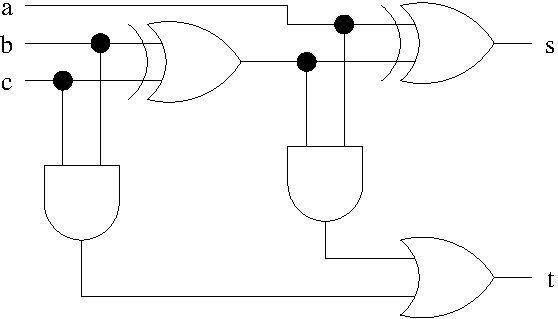
\includegraphics[width=6cm]{add3.pdf}
\end{minipage}\hspace{5mm}
\begin{minipage}{1.5cm}
$$\begin{tabular}{c}
$a\cdot b$\\
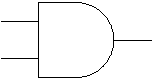
\includegraphics[width=1.25cm]{et.pdf}\\[2mm]
$a+b$\\
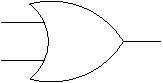
\includegraphics[width=1.25cm]{ou.pdf}\\[2mm]
$a\oplus b$\\
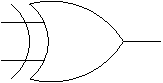
\includegraphics[width=1.25cm]{xor.pdf}
\end{tabular}$$
\end{minipage}$$
\end{td}
}
%------------------------------------------

%------------------------------------------
\begin{frame}
\frametitle{\uppercase{Contrôles}}
\framesubtitle{\uppercase{Evaluations des apprentissages}}
%------------------------------------------
\begin{block}{Contrôle de Laboratoire}
	\begin{itemize}
	\item contrôle sur la préparation des exercices de laboratoire
	\item durée 15' (en début d'une séance de laboratoire)
	%\pause
	\item[$\rightarrow$] \alert{note de contrôle continu de laboratoire  (coefficient 1)}
	\end{itemize}
\end{block}
%\pause

\begin{block}{Contrôle de synthèse}
	\begin{itemize}
	\item contrôle des compétences acquises sur un thème donné
	\item durée 1h30 (en dehors de la grille horaire)
	%\pause
	\item[$\rightarrow$] \alert{1 DS (coefficient 1)}
	\end{itemize}
\end{block}

\end{frame}
\note{
\mbox{}\null\vfill

\begin{td}[Exemple de QCM]
\mbox{}\hfill un seul item correct par question
\begin{enumerate}
\item L'informatique est la science
	\begin{enumerate}
	\item des signaux électriques porteurs d'information ou d'énergie
	\item du mouvement des systèmes matériels et de leurs déformations
	\item du traitement automatique de l'information
	\item de la commande des appareils fonctionnant sans intervention humaine
	\end{enumerate}
\item Le logiciel est
	\begin{enumerate}
	\item la mémoire de l'ordinateur
	\item le traitement automatique de l'information
	\item l'ensemble des données manipulées par les instructions
	\item un ensemble structuré d'instructions décrivant un traitement d'informations
		à faire réaliser par un matériel informatique
	\end{enumerate}
\item La validité d'un algorithme est son aptitude
	\begin{enumerate}
	\item à utiliser de manière optimale les ressources du matériel qui l'exécute
	\item à se protéger de conditions anormales d'utilisation
	\item à calculer le nombre d'instructions élémentaires nécessaires pour
		réaliser la tâche pour laquelle il a été conçu
	\item à réaliser exactement la tâche pour laquelle il a été conçu
	\end{enumerate}
\end{enumerate}

\end{td}
}
%------------------------------------------

%------------------------------------------
\begin{frame}
\frametitle{\uppercase{Notation}}
\framesubtitle{\uppercase{\og 0 ? C'est parfait ! \fg}}
%------------------------------------------
\centerline{note $\equiv$ distance à l'objectif}
\centerline{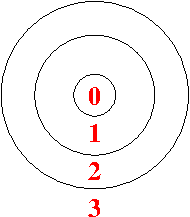
\includegraphics{cible.pdf}}
%\pause

$$\begin{tabular}{l@{ : }l@{ $\rightarrow$ }l}
0 & \og en plein dans le mille !\fg 	& l'objectif est atteint\\
1 & \og pas mal !\fg					& on se rapproche de l'objectif\\
2 & \og tout juste sur la cible !\fg 	& on est encore loin de l'objectif\\
3 & \og même pas touchée !\fg 			& l'objectif n'est pas atteint\\
4 & \og même pas visée !\fg 			& absence
\end{tabular}$$

\end{frame}
\note{
\mbox{}\null\vfill

\begin{rem}[Notation]
Ainsi, et pour changer de point de vue sur la notation, le contrôle 
est réussi lorsqu'on a 0 ! Il n'y a pas non plus de $1/2$ point ou de $1/4$ 
de point : le seul barême possible ne comporte que 4 niveaux : 0, 1, 2 et 3.
On ne cherche donc pas à «~grappiller~» des points : 
\begin{itemize}
\item on peut avoir 0 (objectif atteint) et avoir fait une ou deux erreurs 
	bénignes en regard de l'objectif recherché;
\item on peut avoir 3 (objectif non atteint) et avoir quelques éléments de
	réponse corrects mais sans grand rapport avec l'objectif recherché;
\item on a 4 en cas d'absence.
\end{itemize}
\end{rem}
}
%------------------------------------------

%------------------------------------------
\begin{frame}
\frametitle{\mbox{\uppercase{Evaluation des enseignements}}}
\framesubtitle{\uppercase{Démarche qualité}}
%------------------------------------------
\begin{columns}[T]
\column{5.5cm}
{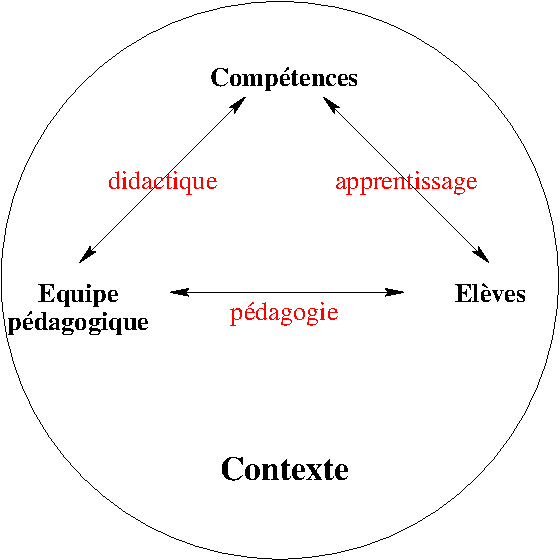
\includegraphics[width=5.5cm]{didac5.pdf}}
%\pause
\column{5.5cm}
\begin{itemize}
\item « contrat pédagogique »
\item 1 évaluation des enseignements par semestre\\
	(sur le site Web)
%\pause
\item améliorer les enseignements
\end{itemize}
\end{columns}
\end{frame}
\note{
{\bf Définitions}\begin{description}
\item[pédagogie] 
	La pédagogie désigne les méthodes et pratiques d'enseignement et 
	d'éducation ainsi que toutes les qualités requises pour transmettre 
	un savoir quelconque.
\item[didactique]
	La didactique se différencie de la pédagogie par le rôle central des contenus 
	disciplinaires et par sa dimension épistémologique (la nature des connaissances à
	enseigner).
\item[apprentissage]
	L'apprentissage est l'acquisition de nouveaux savoirs ou savoir-faire, 
	c'est-à-dire le processus d'acquisition de connaissances, compétences, 
	attitudes ou valeurs, par l'étude, l'expérience ou l'enseignement.
\end{description}
}
%------------------------------------------


%-------------------------------------------------------------------------
\end{document}
%-------------------------------------------------------------------------
